\section{Organiser ses données}
\subsection{Les fichiers : noms et contenu}
\begin{frame}{Un fichier}
  \begin{block}{De l'information au stockage}
    Les informations utilisées dans un ordinateur sont stockées dans la
    \emph{mémoire de masse}, qui se distingue de la \emph{mémoire vive}
    par sa résistance à l'extinction et de la \emph{mémoire morte} (et
    plus tard, du \emph{firmware}) par sa mutabilité.

    Les performances des systèmes de stockage de masse sont meilleures
    chaques années, mais l'ordre de grandeur reste la ms ou 100 µs.
  \end{block}
  \begin{block}{De l'information au fichier}
    L'information est découpée en petites unités qui s'appellent des
    fichiers, sémantiquement cohérentes --- ce sont des informations qui
    « vont ensemble ». Ces éléments de base du stockage informatique
    peuvent ne contenir que très peu d'information ou représenter
    plusieurs Go de données par fichier.

    Un fichier est lié à la façon dont on y accède (son \emph{nom} et
    son \emph{chemin}), mais nous verrons que ce n'est pas un
    identifiant : il peut y avoir plusieurs accès différents à un même
    fichier (\emph{liens}).
  \end{block}
\end{frame}
\begin{frame}{Noms et contenu des fichiers}
  \begin{block}{La décomposition traditionnelle d'un nom de fichier}
    \begin{columns}
      \begin{column}{8cm}
        Deux parties séparées par un point:
        \begin{itemize}
        \item La $1\up{ère}$ partie informe sur la nature du contenu du
          fichier,
        \item La $2\up{ème}$ partie informe sur le format ou la finalité des données.
        \end{itemize}
      \end{column}
      \begin{column}{3cm}
        \begin{tabular}{|r@{}r@{}l|}
          \hline
          {\color{solarizedRed}nom}&.&{\color{solarizedGreen}extension} \\
          {\color{solarizedRed}prefix}&.&{\color{solarizedGreen}suffix} \\
          {\color{solarizedRed}description}&.&{\color{solarizedGreen}format}\\
          \hline
        \end{tabular}
      \end{column}
    \end{columns}
    \begin{itemize}
    \item[\ddialogwarning] Selon les systèmes, certains caractères sont interdits. Par exemple \texttt{*} sous Windows, \texttt{/} sous Linux.
    \end{itemize}
  \end{block}
  \begin{columns}
    \begin{column}{5.5cm}
      \begin{block}{Exemples de noms de fichiers}
        \begin{center}
          \begin{tabular}{ll}
            \hline
            Extension&Contenu\\
            \hline
            .c&Sources C\\
            .html&Document Web\\
            .pdf&Document Mis en page\\
            .txt&Texte brut\\
            \hline
          \end{tabular}
          \vfill
          \begin{tabular}{ll}
            \hline
            Enigmatique&Informatif\\
            \hline
            e3.c&teste\_boucle\_for.c\\
            New.pdf&2011\_IntroSys\_cours\_1.pdf\\
            toto.sh&test\_boucle\_for.sh\\
            \hline
          \end{tabular}
        \end{center}
      \end{block}
    \end{column}
    \begin{column}{5.5cm}
      \begin{alertblock}{Choix des noms}
        \begin{itemize}
        \item[\ddialoginformation] Ils doivent être choisis minutieusement pour être informatifs.
        \item[\ddialogsystem] Choisir un nom : réfléchir pour un gain de temps pour
          retrouver le fichier ou le répertoire concerné.
        \item[\ddialogwarning] Importance de la casse (Linux), tolérance
          ailleurs (OS X, Windows).
        \end{itemize}
      \end{alertblock}
    \end{column}
  \end{columns}
\end{frame}
\subsection{Organisation des données enregistrées}
\begin{frame}{Des fichiers et des répertoires}
  \begin{block}{Les fichiers... en vrac ?}
    Les fichiers sont regroupés dans des répertoires (en anglais
    \emph{directory} ou \emph{folders}). Les répertoires peuvent
    contenir des fichiers ou d'autres répertoires. L'organisation des
    fichiers est réglée par le \emph{système de fichiers}
    (ang. \emph{filesystem}).

    \begin{itemize}
    \item Cette organisation arborescente permet de faciliter la
      recherche d'un fichier,
    \item Les fichiers sont regroupés par application, par thème, par
      format, par fonction, \dots
    \item Organisation \emph{hiérarchique} qui permet d'organiser les données et
      de faciliter leur accès.
    \end{itemize}
  \end{block}
  \begin{columns}
    \begin{column}{.7\linewidth}
      \begin{block}{De très nombreux fichiers et répertoires}
        \begin{itemize}
        \item[\ddialoginformation] Le nombre de fichiers enregistrés sur un disque dur peut
          aisément dépasser 100.000 fichiers,
        \item Dans un même répertoire le nom est un identifiant.
        \item Les répertoires et les fichiers partagent les mêmes noms.
        \item[\dialogwarning] Sous Windows, pas d'extension pour les répertoires.
        \end{itemize}
      \end{block}
    \end{column}%
    \begin{column}{.25\linewidth}
      % 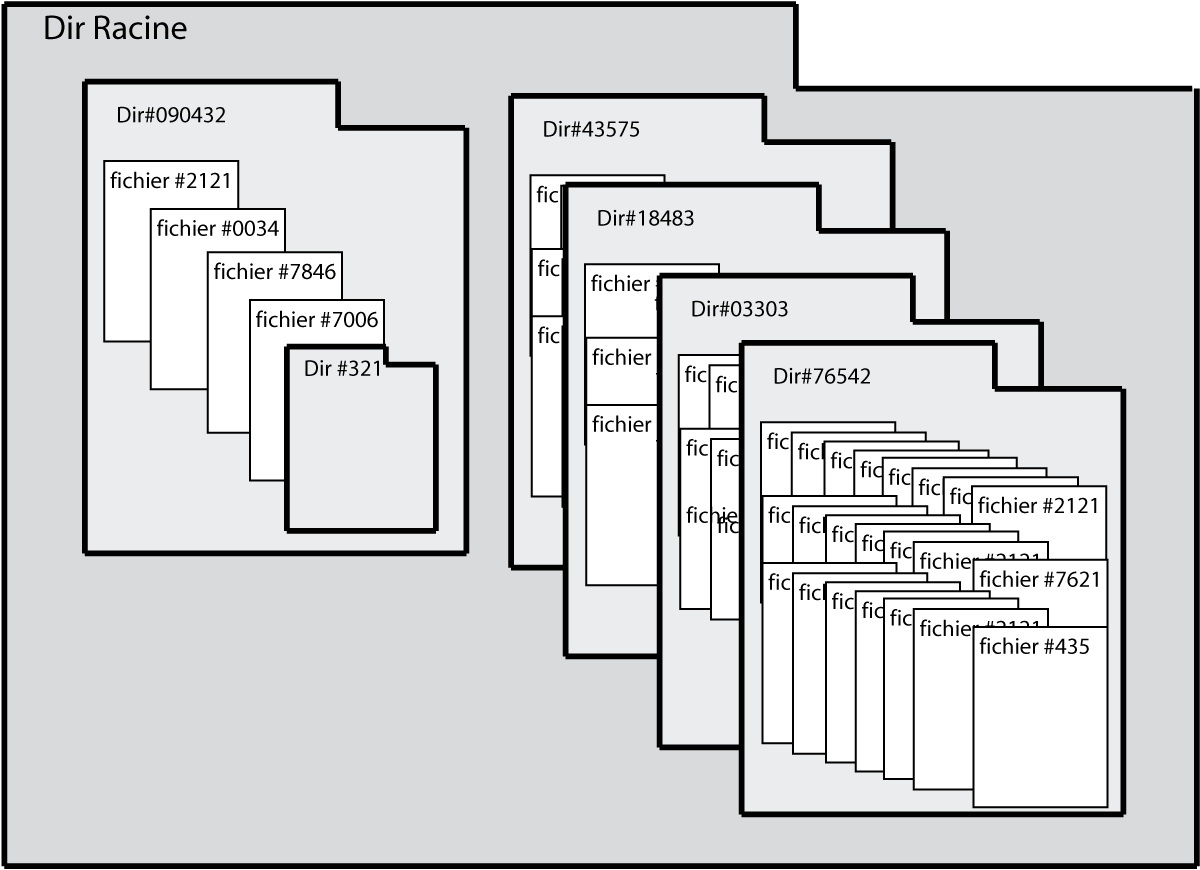
\includegraphics[width=\linewidth]{img/s02/file_system}
      \begin{alertblock}{Remarque}
        \begin{itemize}
        \item[\dialogerror] Avec tous les fichiers au même
          \textit{endroit}, il est très difficile de les lister (trop à
          lire).
        \end{itemize}
      \end{alertblock}
    \end{column}
  \end{columns}
\end{frame}

\subsection{L'organisation arborescente}
\begin{frame}{Exemple d'arborescence Linux}
  \dirtree{%
    .1 \DTd{}\DTfcomment{Répertoire racine \emph{(Root Directory)}}.  .2
    \DTd{bin}.  .3 (\dots).  .2 \DTd{home}.  .3
    \DTd{moi}\DTfcomment{Répertoire personnel \emph{(User
        directory)}}.  .4 \DTd{Mes~Documents}.  .5 ListeDesCourses.txt.
    .5 Exercice\_1.sh.  .4 (\dots).  .3 \DTd{anonymous}.  .4
    LisezMoi.txt.  .4 \DTd{Telechargements}.
    % .5 Cours\_Systeme.pdf.
    .5 (\dots).  .2 (\dots).  }
  \begin{alertblock}{Les répertoires importants}
    \begin{itemize}
    \item La \textbf{racine} (\textit{Root directory}) contient tous
      les répertoires et fichiers accessibles depuis le système.
    \item Le \textbf{répertoire personnel} (\textit{User Directory} ou
      \textit{Home Directory}) est le répertoire dans lequel
      l'utilisateur peut faire ce qu'il veut (écrire, modifier,
      supprimer, installer \dots).
    \end{itemize}
  \end{alertblock}
\end{frame}
\subsection{La notion de chemin}
\begin{frame}{La notion de chemin}
  \begin{block}{Le chemin définit un accès unique à partir de la racine}
    \begin{itemize}
    \item Deux fichiers ou répertoires ne peuvent pas porter le même nom
      si ils sont dans un même répertoire.
    \item Sous Linux, les noms des fichiers et répertoires différencient
      les caractères \textsc{Majuscules} et minuscule. Les fichiers
      \alert{E}ssai.txt et \alert{e}ssai.txt peuvent donc être dans le
      même répertoire.
    \end{itemize}
  \end{block}
  \begin{block}{Exemples de chemins absolus}
    \dirtree{%
      .1 \DTd{}\DTfcomment{Un chemin absolu part de la racine {\color{solarizedAccent}/}}.
      .2 \DTd{home}\DTfcomment{/{\color{solarizedAccent}home/}}.
      .3 \DTd{moi}\DTfcomment{/home/{\color{solarizedAccent}moi/}}.
      .4 \DTd{Etoiles}\DTfcomment{/home/moi/{\color{solarizedAccent}Etoiles/}}.
      .5 SOLEIL.jpg\DTfcomment{/home/moi/Etoiles/{\color{solarizedAccent}SOLEIL.jpg}}.
      .5 Soleil.jpg\DTfcomment{/home/moi/Etoiles/{\color{solarizedAccent}Soleil.jpg}}.
      .4 \DTd{Systeme\_Solaire}\DTfcomment{/home/moi/{\color{solarizedAccent}Systeme\_Solaire/}}.
      .5 SOLEIL.jpg\DTfcomment{/home/moi/Systeme\_Solaire/{\color{solarizedAccent}SOLEIL.jpg}}.
    }
  \end{block}
  \begin{alertblock}{Syntaxe d'un chemin absolu}
    Le chemin \textit{absolu} d'un élément du système de fichier est
    unique (sauf avec un \emph{lien}). Il donne la liste des répertoires
    et sous-répertoires en partant de la racine \lin{/} (la référence de
    l'arborescence) jusqu'à la cible.
  \end{alertblock}
\end{frame}

% MOVE TO 03
% \begin{frame}{La notion de partition}
%   \begin{block}{Windows : les partitions visibles}
%     Le ou les disques sont découpés en systèmes de fichiers indépendants
%     qui sont numérotés par des lettres. A et B sont réservés au lecteur
%     de disquette, C au disque système. Nombre limité de partitions.

%     Les partitions aident à l'organisation des données par type
%     (système, utilisateurs, sauvegarde).
%   \end{block}
%   \begin{block}{Unix : les partitions invisibles}
%     Sous Unix et ses variantes (OS X et Linux), la partition racine est
%     celle qui contient le système. Les autres partitions sont
%     \emph{montées} à la place d'un répertoire et sont en quelque sortes
%     greffées dans l'arbre qui reste unique. La racine de la partition
%     montée prend la place du répertoire dans l'arborescence.
%   \end{block}
% \end{frame}

\subsection{Répertoire courant et chemins relatifs}
\begin{frame}{Répertoire courant et chemins relatifs}
  \begin{block}{Le répertoire courant}
    \begin{itemize}
    \item Le répertoire courant est un répertoire de référence d'où sont
      lancées les commandes du shell.
    \item Par défaut, le répertoire courant est le répertoire personnel
      de l'utilisateur,
    \item Naviguer dans l'arborescence équivaut à modifier le répertoire
      courant.
    \end{itemize}
  \end{block}
  \begin{block}{Exemples de chemins relatifs}
    \dirtree{%
      .1 \DTd{home}\DTfcomment{../..}.
      .2 \DTd{moi}\DTfcomment{../}.
      .3 \DTd{Etoiles}\DTfcomment{{\color{solarizedRed}Répertoire Courant ~~./}}.
      .4 SOLEIL.jpg\DTfcomment{SOLEIL.jpg {\color{black}ou} ./SOLEIL.jpg}.
      .4 Antares.jpg\DTfcomment{Antares.jpg {\color{black}ou} ./Antares.jpg}.
      .3 \DTd{Systeme\_Solaire}\DTfcomment{../Systeme\_Solaire/}.
      .4 terre.gif\DTfcomment{../Systeme\_Solaire/terre.gif}.
    }
  \end{block}
  \begin{alertblock}{Syntaxe d'un chemin relatif}
    \begin{itemize}
    \item Le chemin \textit{relatif} d'un fichier ou d'un répertoire donne la liste des répertoires et sous-répertoires en partant du répertoire courant (la référence \textit{relative} dans l'arborescence) jusqu'à la cible.
    \item Il est relatif, car lorsque le répertoire courant change, le chemin relatif change.
    \end{itemize}
  \end{alertblock}
\end{frame}
% MOVE TO 03
% \begin{frame}{Chemin canonique}
%   \begin{block}{Chemin canonique}
%     Le chemin qui part de la racine et n'emprunte aucun \emph{lien symbolique} (une forme de lien que nous verrons plus loin) ni aucun \emph{lien parent} (raccourci \lin{..} vers un répertoire parent d'un autre) est appelé le chemin \emph{canonique absolu}.
%   \end{block}
% \end{frame}
%%%%%%%%%%%%%% 
\subsection{Notation spéciales}
\begin{frame}{Notation spéciales}
  \begin{block}{Les chemins des répertoires de référence}
    \begin{columns}
      \begin{column}{6cm}
        \begin{center}
          \begin{tabular}{lr}
            \hline
            Répertoire&Notation\\
            \hline
            Répertoire racine&\lin{/}\\
            Répertoire personnel&\lin{\~{}}\\
            \hline
          \end{tabular}
        \end{center}
      \end{column}
      \begin{column}{6cm}
        \begin{center}
          \begin{tabular}{lr}
            \hline
            Répertoire&Notation\\
            \hline
            Répertoire courant&\lin{.}\\
            Répertoire parent&\lin{..}\\
            \hline
          \end{tabular}
        \end{center}
      \end{column}
    \end{columns}
    \begin{itemize}
    \item[\ddialogwarning] La notation \lin{\~{}} est un chemin
      absolu, remplacée par le vrai chemin avant l'exécution des
      commandes. C'est un raccourci \emph{au niveau du shell, pas au
        niveau du système d'exploitation}.
    \end{itemize}
  \end{block}
  \begin{block}{Exemple de chemins valides pointant le fichier cible}
    \begin{columns}
      \begin{column}{55mm}
        \dirtree{%
          .1 \DTd{}\DTfcomment{{\color{solarizedAccent}Répertoire Racine}}.
          .2 \DTd{home}.
          .3 \DTd{moi}\DTfcomment{{\color{solarizedAccent}Répertoire Personnel}}.
          .4 \DTd{Etoiles}\DTfcomment{{\color{solarizedAccent}Répertoire Courant}}.
          .5 Soleil.jpg\DTfcomment{Fichier cible}.
        }
      \end{column}
      \begin{column}{7cm}
        \begin{center}
          \footnotesize{
            \begin{tabular}{l}
              \hline
              Chemins Absolus\\
              \hline
              \lin{/home/moi/Etoiles/Soleil.jpg}\\
              \lin{\~{}/Etoiles/Soleil.jpg}\\
              \lin{/home/moi/../moi/Etoiles/Soleil.jpg}\\
              \lin{/home/moi/../../home/moi/Etoiles/Soleil.jpg}\\
              \hline
              Chemins Relatifs\\
              \hline
              \lin{Soleil.jpg}\\
              \lin{./Soleil.jpg}\\
              \lin{../Etoiles/Soleil.jpg}\\
              \lin{../../moi/Etoiles/./Soleil.jpg}\\
            \end{tabular}
          }
        \end{center}
      \end{column}
    \end{columns}	
  \end{block}
\end{frame}

\begin{frame}{L'archivage}
  \begin{block}{D'une arborescence à un fichier}
    Une technique souvent utilisée consiste à transformer une partie de
    l'arborescence en un fichier qui n'est pas utilisable directement. Ce
    fichier peut ensuite être retransformé en une arborescence.
  \end{block}
  \begin{columns}
    \begin{column}{55mm}
      \begin{block}{Le format tar}
        Utilisé depuis les années 80, le format tar est un pilier du
        monde Unix. Il est parfaitement libre. Il servait initialement
        aux sauvegardes sur bande magnétique (\emph{t}ape
        \emph{ar}chive).
        
        Le format tar ne permet pas la compression, mais la commande
        \lin{tar} donne accès à des programmes de compression qui
        permettent de réduire la taille de l'archive. Une archive au
        format tar est appelée un(e) \emph{tarball}.

        Le compresseur le plus connu est \lin{gzip} dont les fichiers
        compressés ont un suffixe \lin{.gz}. Souvent on combine les deux
        suffixes : une archive compressée peut ainsi s'appeler
        \lin{textes2015.tar.gz} ou \lin{textes2015.tgz}.
      \end{block}
    \end{column}
    \begin{column}{55mm}
      \begin{block}{Le format zip}
        Principalement utilisé pour son universalité depuis 1986, le format zip est
        plus ou moins libre (il y a des doutes sur la possibilité de
        brevet sur les techniques employées). Le format zip n'est pas
        uniquement caractérisé par son extension : plusieurs autres
        formats de fichier sont en fait une archive ZIP qui contient
        divers documents (par exemple, un fichier \lin{docx} pour
        Microsoft Word est en fait un ZIP qui contient divers fichiers
        XML et images).

        Le format zip, en plus de l'archivage permet aussi la
        compression. La commande \lin{zip}/\lin{unzip} doit donc
        permettre la décompression.
      \end{block}
    \end{column}
  \end{columns}
\end{frame}

\subsection{Quelques mini-manuels}
\begin{frame}{Conventions}
  \begin{block}{Noms et chemins}
    \begin{itemize}
    \item Un chemin peut être absolu ou relatif. Il peut utiliser les notations spéciales.
    \item Par convention la notion de fichier sera comprise dans son sens large. Par exemple, le chemin d'un fichier devra être interprété sans distinction comme le chemin vers un fichier ordinaire ou comme le chemin vers un répertoire (sauf mention contraire explicite).
    \end{itemize}
  \end{block}
  \begin{block}{Commandes, options, paramètres}
    \begin{description}
    \item[Commande] c'est le nom d'un programme qui exécute une action.
    \item[Options] ce sont des paramètres optionnels. Ils peuvent être
      omis. L'ajout d'options modifie le comportement de la commande (le
      résultat). Les options sont montrées encadrées par les caractères
      \lin{[ ... ]} (qu'il ne faut pas mettre).
    \item[Paramètres] ce sont des arguments que la commande évalue.
    \end{description}
  \end{block}
  \begin{block}{Sources et destination}
    Les commandes de déplacement acceptent une ou des \emph{sources} qui
    sont des fichiers ou répertoires d'origine, et une
    \emph{destination} qui est un fichier ou un répertoire.
  \end{block}
\end{frame}
\begin{frame}{Manipulation de l'arborescence en ligne de commande}
  \begin{columns}
    \begin{column}{4cm}
      \begin{block}{Alternatives pour naviguer dans l'arborescence et
          manipuler les fichiers}
        \begin{center}
          Interface Graphique\\
          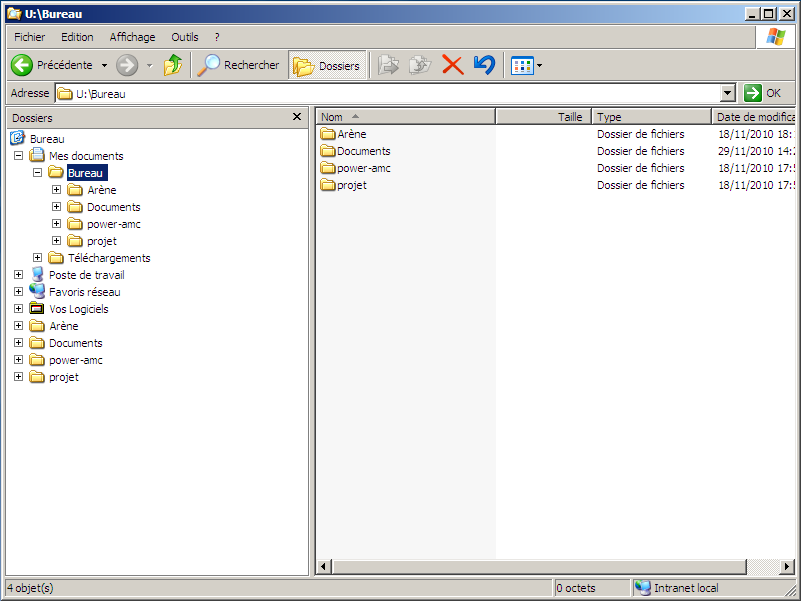
\includegraphics[height=2cm]{img/s02/explorer_windows.png}
        \end{center}
        \begin{center}
          Ligne de Commande\\
          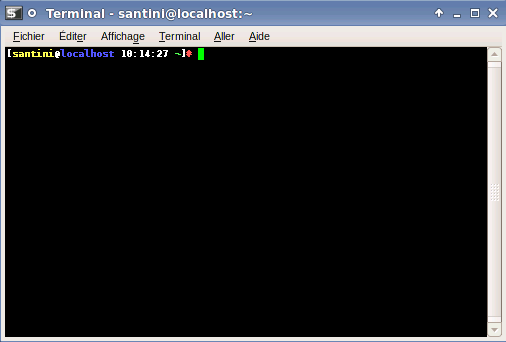
\includegraphics[height=2cm]{img/s02/terminal_single.png}
        \end{center}
      \end{block}
    \end{column}
    \begin{column}{75mm}
      \begin{block}{Boîte à outils : manipuler l'arborescence}
        \begin{center}
          \begin{tabular}{ll}
            \hline
            Commande&Fonction principale\\
            \hline
            \lin{pwd}&Afficher le nom du répertoire courant\\
            \lin{cd}&Changer de répertoire courant\\
            \lin{ls}&Afficher le contenu d'un répertoire\\
            \lin{cat}&Afficher le contenu d'un fichier\\\hline
            \lin{touch}&Créer un fichier\\
            \lin{mkdir}&Créer un répertoire\\\hline
            \lin{rm}&Supprimer fichier(s) ou répertoire(s) \\
            \lin{cp}&Copier fichier(s) ou répertoire(s)\\
            \lin{mv}&Déplacer/Renommer fichier(s) ou répertoire(s)\\
            \hline
          \end{tabular}
        \end{center}
      \end{block}
    \end{column}
  \end{columns}
\end{frame}
\manpage{pwd} \manpage{cd}
\manpage{ls} \manpage{ls(bis)} \manpage{cat}
\manpage{touch} \manpage{mkdir} \manpage{mkdir(bis)}
\manpage{rm} \manpage{rm(bis)} \manpage{cp}
\manpage{cp(bis)} \manpage{cp(ter)} \manpage{mv} \manpage{mv(bis)}
\manpage{mv(ter)}
\manpage{tar}\manpage{tar(bis)}

\begin{exercice}
  \begin{exercicelet}{Préparation}
    \begin{questions}
    \item Ouvrez un terminal. Vérifiez que le répertoire dans lequel
      vous êtes est bien \lin{/home/usager/123456789/}. Quelle est la
      commande qui permet de le faire ? (123456789 = votre identifiant)
    \item Vérifiez le contenu du répertoire \lin{Documents} qui est dans
      votre répertoire personnel. Quelle est la commande qui permet de
      le faire ? Est-ce qu'il y a quelque chose ?
    \item Faites la vérification de trois façons différentes : chemin
      absolu, utilisation du raccourci \lin{\~}, utilisation d'un chemin
      relatif.
    \item Changez le répertoire courant pour aller dans
      \lin{Documents}. Quelle est la commande pour le faire ?
    \item Créez en ligne de commande un répertoire \lin{m1101} dans
      \lin{\~/Documents}. À partir de maintenant, assurez-vous que le
      répertoire courant est ce répertoire \lin{m1101}.
    \item Téléchargez l'archive contenant les données pour ce TP:
      Allez sur la page
      \url{http://lipn.fr/~dubacq/m1101.html}.
      Téléchargez le fichier \lin{photos.tar}. Recherchez où
      le fichier a été écrit dans l'arborescence de votre répertoire
      personnel.
    \item Donnez la (suite de) commande(s) permettant de déplacer le
      fichier d'archive dans le répertoire \lin{m1101} que vous venez de
      créer. À la fin des commandes, le répertoire \lin{m1101} sera
      toujours votre répertoire courant et ne contiendra que le fichiers
      photos.tar.
    \item Quelle commande permet de vérifier que l'archive est bien dans
      le répertoire \verb|~/Documents/m1101|?
    \end{questions}
  \end{exercicelet}
\end{exercice}
\begin{exercice}
  \begin{exercicelet}{Examen de fichiers}
    \begin{questions}
    \item Quelles sont les informations données par le nom du fichier?
    \item\label{qsee} Les commandes \texttt{less}, \texttt{cat} et \texttt{hexdump} permettent
      d'afficher le contenu d'un fichier. Analysez la différence de
      comportement entre ces deux commandes sur le fichier
      \lin{photos.tar}. Qu'en concluez-vous? Quel est le programme le
      plus adapté pour voir le contenu de ce fichier ?
      \begin{correction}
        cat affiche brutalement du binaire sans filtrer
        (incompréhensible), less propose une interface (mais ça reste du
        binaire dans la configuration par défaut de Debian), hexdump
        transforme le binaire en hexadécimal (ce n'est pas beaucoup plus
        lisible). Le programme le plus adapté est donc... tar, comme
        montré dans la question suivante ! Avec \texttt{tar tf
          photos.tar} on obtient la liste des fichiers.
      \end{correction}
    \item Relisez le manuel de la commande \texttt{tar}. Vérifiez la
      liste des fichiers contenus dans l'archive. Combien y en a-t-il ?
    \item Sortez les fichiers de l'archive.
      \begin{correction}
        tar xf photos.tar
      \end{correction}
    \item Avec les commandes de la question~\ref{qsee}, regardez le
      fichier contenu dans un répertoire. Analysez la différence de
      comportement entre ces commandes. Qu'en concluez-vous?
      \begin{correction}
        La commande less est plus adaptée (pagination, arrêt par la
        touche q). La commande hexdump continue de produire de
        l'hexadécimal (on peut montrer hexdump -C aux curieux).
      \end{correction}
    \end{questions}
    
    Remarques: si un affichage prend trop de temps, utilisez le
    raccourci clavier adéquat pour suspendre l'exécution de la commande
    courante.  Si l'affichage de votre terminal est durablement
    perturbé, dans le menu Terminal \textrightarrow Réinitialiser le
    terminal.
  \end{exercicelet}
\end{exercice}
\subsection{Métacaractères}
\begin{frame}{Le métacaractère \lin{*}}
  \begin{block}{Le caractère \lin{*}}
    \begin{itemize}
    \item[\ddialogsystem] Le shell traduit la ligne de commande en \texttt{commande argument1
        argument2 ...}. Avant l'exécution, il traduit certains caractères
      selon des règles précisées ici.
    \item Le cataractère \lin{*} est utilisé comme un \textit{joker}
      pour remplacer une chaîne de caractères,
    \item Il est utilisé dans un chemin pour pointer plusieurs fichiers
      ou répertoires existants dont le chemin partage un motif commun.
    \item Le caractère \lin{*} peut être n'importe où dans le chemin,
      plusieurs fois si nécessaire.
    \end{itemize}
  \end{block}
  \begin{block}{Exemple de manipulation avec la commande \lin{mv}}
    \scriptsize{
      \begin{columns}
        \begin{column}{6cm}
          \begin{center}
            \mpromptS{%
              \promptS{mv *.jpg Images/}{} }
          \end{center}
        \end{column}
        \begin{column}{6cm}
          Ici, le chemin \lin{*.jpg} pointe tous les fichiers du
          répertoire courant dont le nom se fini par l'extension
          \lin{.jpg}. Il pointe donc les fichiers \lin{etacentauri.jpg}
          et \lin{aldebaran.jpg} et exclue les autres fichiers (ici le
          fichier \lin{alphacentauri.gif}).
        \end{column}
      \end{columns}
      \begin{columns}
        \begin{column}{6cm}
          \dirtree{%
            .1
            \DTd{{\color{solarizedRed}moi}}\DTfcomment{{\color{solarizedRed}Répertoire
                Courant}}.  .2 aldebaran{\color{solarizedGreen}.jpg}
            \DTfcomment{{\color{solarizedGreen}Fichier ciblé}}.  .2
            alphacentauri.gif .  .2
            etacentauri{\color{solarizedGreen}.jpg}
            \DTfcomment{{\color{solarizedGreen}Fichier ciblé}}.  .2
            \DTd{{\color{solarizedBlue}Images}}\DTfcomment{{\color{solarizedBlue}Répertoire
                final}}.  }
        \end{column}
        \begin{column}{6cm}
          \dirtree{%
            .1
            \DTd{{\color{solarizedRed}moi}}\DTfcomment{{\color{solarizedRed}Répertoire
                Courant}}.  .2 alphacentauri.gif .  .2
            \DTd{{\color{solarizedBlue}Images}}\DTfcomment{{\color{solarizedBlue}Répertoire
                final}}.  .3 {\color{solarizedGreen}aldebaran.jpg}
            \DTfcomment{{\color{solarizedGreen}Fichier déplacé}}.  .3
            {\color{solarizedGreen} etacentauri.jpg}
            \DTfcomment{{\color{solarizedGreen}Fichier déplacé}}.  }
        \end{column}
      \end{columns}
    }
  \end{block}
\end{frame}
\begin{frame}{Exemples d'utilisation de l'étoile}
  \begin{block}{Utilisation simple avec la commande \lin{mv}}
    \scriptsize{
      \begin{columns}
        \begin{column}{6cm}
          \begin{center}
            \mpromptS{%
              \promptS{mv al* Images/}{} }
          \end{center}
        \end{column}
        \begin{column}{6cm}
          Ici, le chemin \lin{al*} pointe tous les fichiers du
          répertoire courant dont le nom commence par les caractères
          \lin{al}. Il pointe donc les fichiers \lin{aldebaran.jpg} et
          \lin{alphacentauri.gif} et exclue les autres fichiers (ici le
          fichier \lin{etacentauri.jpg}).
        \end{column}
      \end{columns}
      \begin{columns}
        \begin{column}{6cm}
          \dirtree{%
            .1
            \DTd{{\color{solarizedRed}moi}}\DTfcomment{{\color{solarizedRed}Répertoire
                Courant}}.  .2 {\color{solarizedGreen}al}debaran.jpg
            \DTfcomment{{\color{solarizedGreen}Fichier ciblé}}.  .2
            {\color{solarizedGreen}al}phacentauri.gif
            \DTfcomment{{\color{solarizedGreen}Fichier ciblé}}.  .2
            etacentauri.jpg.  .2
            \DTd{{\color{solarizedBlue}Images}}\DTfcomment{{\color{solarizedBlue}Répertoire
                final}}.  }
        \end{column}
        \begin{column}{6cm}
          \dirtree{%
            .1
            \DTd{{\color{solarizedRed}moi}}\DTfcomment{{\color{solarizedRed}Répertoire
                Courant}}.  .2 etacentauri.jpg .  .2
            \DTd{{\color{solarizedBlue}Images}}\DTfcomment{{\color{solarizedBlue}Répertoire
                final}}.  .3 {\color{solarizedGreen}aldebaran.jpg}
            \DTfcomment{{\color{solarizedGreen}Fichier déplacé}}.  .3
            {\color{solarizedGreen}alphacentauri.gif}
            \DTfcomment{{\color{solarizedGreen}Fichier déplacé}}.  }
        \end{column}
      \end{columns}
    }
  \end{block}
  \begin{block}{Utilisation double avec la commande \lin{mv}}
    \scriptsize{
      \begin{columns}
        \begin{column}{6cm}
          \begin{center}
            \mpromptS{%
              \promptS{mv *centauri* JPG/}{} }
          \end{center}
        \end{column}
        \begin{column}{6cm}
          Ici, le chemin \lin{*centauri*} pointe tous les fichiers du
          répertoire courant dont le nom contient la chaîne de
          caractères \lin{centauri}. Il pointe donc les fichiers
          \lin{alphacentauri.gif} et \lin{etacentauri.jpg} et exclue les
          autres fichiers (ici le fichier \lin{aldebaran.jpg}).
        \end{column}
      \end{columns}
      \begin{columns}
        \begin{column}{6cm}
          \dirtree{%
            .1
            \DTd{{\color{solarizedRed}moi}}\DTfcomment{{\color{solarizedRed}Répertoire
                Courant}}.  .2 aldebaran.jpg .  .2
            alpha{\color{solarizedGreen}centauri}.gif
            \DTfcomment{{\color{solarizedGreen}Fichier ciblé}}.  .2
            eta{\color{solarizedGreen}centauri}.jpg
            \DTfcomment{{\color{solarizedGreen}Fichier ciblé}}.  .2
            \DTd{{\color{solarizedBlue}Images}}\DTfcomment{{\color{solarizedBlue}Répertoire
                Final}}.  }
        \end{column}
        \begin{column}{6cm}
          \dirtree{%
            .1
            \DTd{{\color{solarizedRed}moi}}\DTfcomment{{\color{solarizedRed}Répertoire
                Courant}}.  .2 aldebaran.jpg .  .2
            \DTd{{\color{solarizedBlue}Images}}\DTfcomment{{\color{solarizedBlue}Répertoire
                final}}.  .3 {\color{solarizedGreen}alphacentauri.gif}
            \DTfcomment{{\color{solarizedGreen}Fichier déplacé}}.  .3
            {\color{solarizedGreen}etcentauri.jpg}
            \DTfcomment{{\color{solarizedGreen}Fichier déplacé}}.  }
        \end{column}
      \end{columns}
    }
  \end{block}
\end{frame}
\begin{frame}{Métacaractère et chemins ciblés}
  \begin{block}{Exemple plus complexe et détails de l'interprétation}
    \begin{itemize}
    \item Le cararctère \lin{*} est développé lors de l'interprétation.
    \end{itemize}
  \end{block}
  \begin{center}
    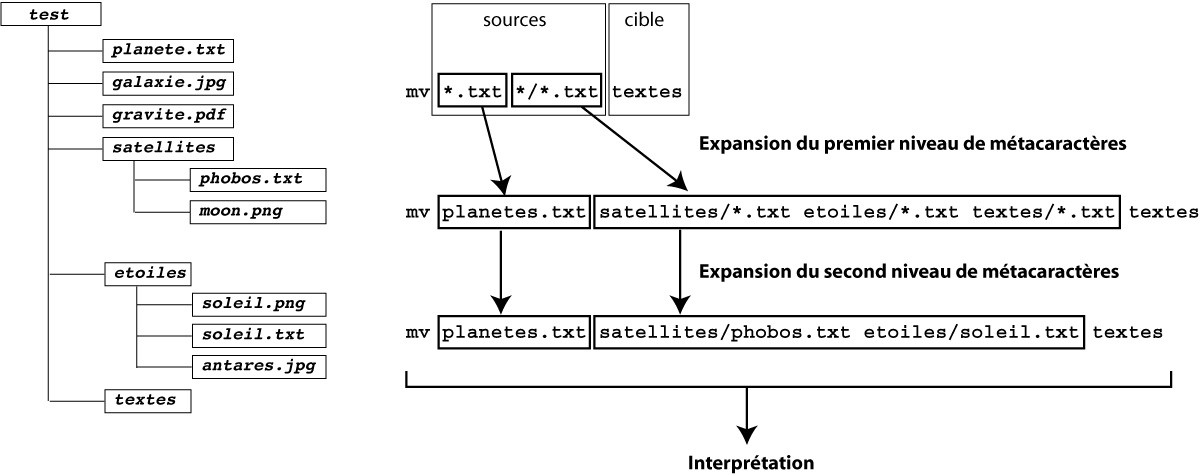
\includegraphics[width=12cm]{img/s02/star_met_mv_interp.jpg}
  \end{center}
\end{frame}
\begin{frame}{Autres métacaractères}
  \begin{alertblock}{Du shell aux programmes}
    Il faut bien se souvenir que les métacaractères sont interprétés par le shell. Cela a deux conséquences :
    \begin{itemize}
    \item Le programme appelé ne sait pas si les noms ont été tapés en entier ou si des métacaractères ont été utilisés. Il n'a que le résultat final.
    \item Dans un programme, on ne peut pas utiliser les métacaractères.
    \end{itemize}
  \end{alertblock}
  \begin{block}{Les jokers}
    Ce sont des motifs simples. Lorsqu'ils ne peuvent pas être
    instanciés, ils ne sont pas supprimés, mais passés tels
    quels. Exemple : \lin{mkdir -p toto/*} selon que \texttt{toto} est
    un répertoire non-vide ou autre chose.

    On y trouve \lin{?} qui remplace une lettre, \lin{[a-c][0-2]} qui remplace a0 b0 c0 a1 b1 c1 a2 b2 c2, 

  \end{block}
  \begin{block}{Les raccourcis}
    Le motif \lin{\{fourch,brou\}ette} est remplacé par
    \lin{fourchette} et \lin{brouette} indépendamment de
    l'existence ou nom de chemins correspondants.
    
    Le motif \lin{\~} a déjà été vu et est remplacé par le chemin absolu
    du répertoire personnel de l'utilisateur courant. \lin{\~{}user} est
    remplacé de la même façon mais pour l'utilisateur \emph{user}.
  \end{block}
\end{frame}
\begin{exercice}
  \begin{exercicelet}{Copie et déplacement}
    \begin{questions}
    \item Quelle commande permet la création "simultanée" de trois
      répertoires \lin{GIF} et \lin{Photos/Portugal},
      \lin{Photos/Marseille} et \lin{Photos/Montagne} ?
    \item Quelle commande permet de \emph{déplacer} depuis le répertoire
      \lin{images} tous les fichiers présentant l'extension
      \lin{gif} dans le répertoire \lin{GIF} nouvellement créé?
    \item Quelle commande permet de \emph{copier} depuis le répertoire
      \lin{images} tous les fichiers présentant l'extension
      \lin{jpg} dans le répertoire \lin{Photos} nouvellement créés?
    \item Définissez le répertoire \lin{Photos/Montagne} comme votre répertoire
      courant. Quelle commande permet de déplacer la photo de chalet dans ce répertoire ?
    \item En vous mettant dans \lin{Photos}, déplacez les photos
      restantes dans le bon répertoire (Marseille est supérieure à
      2000). Si possible, faites usages de jokers.
    \end{questions}
  \end{exercicelet}
\end{exercice}
\begin{exercice}
  \begin{exercicelet}{Suppressions}
    \begin{questions}
    \item Quel est le résultat de la séquence de commandes suivante :
\begin{verbatim}
 cd ..
 rm images
\end{verbatim}
    \item Comment modifier la dernière commande pour supprimer le
      répertoire \texttt{images/}? Comment modifier la commande pour
      éviter les invites de confirmation?
    \item Quelle commande permet de copier le répertoire \texttt{GIF} et
      son contenu dans un répertoire nommé \verb|images_GIF|?
    \item Quelle est la différence entre les deux commandes suivantes:
\begin{verbatim}
      cd ~
      cd /home/usager/votre_identifiant/
\end{verbatim}
    \item Fabriquez une archive qui contient le répertoire Photos (et
      uniquement celui-ci). Vérifiez son contenu.
    \end{questions}
  \end{exercicelet}
  % ----------------limite approximative de cours
\end{exercice}

\subsection{Arborescence et montage}
\begin{frame}{Le partitionnement}
  \begin{block}{Du disque aux partitions}
    \begin{itemize}
    \item Un disque est souvent divisé en plusieurs zones d'usage
      distinct (par exemple, système et données utilisateurs).
    \item Chacun de ces zones est appelée une \emph{partition}. Elle
      est un système de fichiers indépendant des autres, et peut être
      combinée avec d'autres.
    \item Sous Windows, chaque partition est désignée par une lettre
      en fonction de son ordre de découverte par le système. Cette
      lettre fait partie du chemin.
    \item[\dialogwarning] L'ordre des partitions peut changer et donc
      la lettre ; ça pose problème pour les mises à jour.
    \end{itemize}
  \end{block}
  \begin{block}{Montage et démontage}
    \begin{itemize}
    \item Un système d'exploitation peut rendre accessible une
      partition : c'est le \emph{montage} de la partition.
    \item Inversement : c'est le \emph{démontage} de la partition.
    \item[\dialogsystem] Une partition montée peut être utilisée
      normalement par les programmes.
    \item[\dialogerror] Une partition démontée doit utiliser une
      interface spéciale plus compliquée qui contourne le \emph{système
        de fichiers} et permet d'accéder directement au disque.
    \end{itemize}
  \end{block}
\end{frame}
\begin{frame}{Les partitions sous Linux}
  \begin{block}{L'arbre unique}
    \begin{itemize}
    \item Sous Linux, les partitions sont toutes dans regroupés dans une seule arborescence.
    \item[\ddialogsystem] Les partitions qui ne sont pas la racine sont accrochées dans
      la partition racine (ou une autre déjà accrochée) au niveau d'un
      répertoire qui sert de \emph{point de montage}.
    \item[\ddialogerror] Le contenu du point de montage est alors
      inaccessible et remplacé par le contenu du système de fichier qui
      a été monté
    \item Le chemin absolu d'un élément du système monté est le chemin
      du point de montage suivi du chemin dans le système de fichiers
      monté.
    \item[\ddialoginformation] Exemple: fichier \texttt{moi/toto.txt}
      dans un système monté sur \texttt{/home}, le chemin absolu est
      \texttt{/home/moi/toto.txt}.
    \end{itemize}
  \end{block}
  \begin{block}{Le pseudo-système \texttt{/dev}}
    Sous Linux, les périphériques sont accessibles par une interface de
    type fichier. Leur chemin est \texttt{/dev/codeperipherique}. 

    Le sous-arbre à partir de \texttt{/dev} est un système de fichiers
    indépendant d'un périphérique physique. On parle de \emph{système de
      fichiers virtuel}.
  \end{block}
\end{frame}

\manpage{mount}

\begin{exercice}
  \begin{exercicelet}{Analyse de périphériques}
    \begin{questions}
    \item Le périphérique \texttt{zero} est un périphérique virtuel. La
      commande \texttt{dd if=/dev/zero count=1 | hexdump -v} permet de
      voir les 512 premiers octets de ce périphérique virtuel (en
      hexadécimal). Regardez-le. Qu'est-ce qu'il a de particulier ?
      \begin{correction}
        Ce périphérique virtuel n'emet que des octets dont la valeur est
        zéro. Un nombre infini d'octets. L'utilité ne paraît pas très
        évidente, mais ce n'est pas compliqué à faire. Un périphérique
        virtuel est en fait un programme (plus précisément, un morceau
        de ce qu'on appelle le noyau du système d'exploitation) qui
        réagit comme un périphérique, sauf qu'il ne correspond à aucune
        interface physique particulière. Le noyau le considère comme
        s'il existait quelque part un disque infini qui ne contient que
        des zéros.
      \end{correction}
    \item Le périphérique \texttt{urandom} est un périphérique
      virtuel. La commande \texttt{dd if=/dev/urandom count=1 | hexdump
        -v} permet de voir les 512 premiers octets de ce périphérique
      virtuel (en hexadécimal). Regardez-le. Recommencez. Qu'est-ce
      qu'il a de particulier ?
      \begin{correction}
        Ce périphérique virtuel émet des octets ayant une valeur au
        hasard (entre 0 et 255 donc, ou 0 à FF en hexadécimal). Un
        nombre infini d'octets. L'utilité paraît un peu meilleure que
        /dev/zero, puisqu'on imagine bien que des programmes puissent
        demander un accès à une source de données aléatoires (par
        exemple, pour simuler un dé).
      \end{correction}
    \item Le périphérique \texttt{sda1} est une des partitions du disque
      dur. La commande \texttt{dd if=/dev/sda1 count=1 | hexdump -v}
      permet de voir les 512 premiers octets de ce périphérique virtuel
      (en hexadécimal). Regardez-le. Que se passe-t-il ? Un programme
      normal comme \lin{dd} peut-il examiner le disque dur en
      outrepassant le système de fichiers ?
      \begin{correction}
        Ce coup-ci, c'est un vrai périphérique (c'est la partition
        /boot, si je ne me trompe pas sur l'installation du CRIT). Mais
        ils n'ont pas le droit de le consulter ! En effet, l'interface
        d'accès hors-système de fichiers est réservé à des programmes
        spéciaux (comprendre lancés par l'utilisateur root) de façon à
        éviter les mauvaises manipulations qui peuvent découler de
        manipulations non cadrées des données du disque.
      \end{correction}
    \item En utilisant la commande \lin{mount}, analysez les différentes
      partitions présentes dans votre système. Identifiez celles qui
      correspondent à un vrai périphérique et les systèmes de fichier
      virtuel.
      \begin{correction}
        Il n'y a a priori que / et /boot qui sont de vraies partitions
        d'un vrai disque dur local, et /home qui est une partition
        exportée à travers le réseau (par le protocole nfs4).
      \end{correction}
    \end{questions}
  \end{exercicelet}
\end{exercice}

\begin{frame}{Espace libre}
  Une partition occupe une taille fixe. La plupart des systèmes de
  fichiers sont \textbf{de taille fixe}. Elles peuvent accueillir
  uniquement une certaine quantité de données.
  \begin{alertblock}{L'espace de travail}
    Comme dans un parking, la quantité de données que l'on peut mettre
    dans un disque ne doit pas être égale à la quantité de données qu'il
    peut accueillir, sinon, on ne peut pas faire un certain nombre
    d'opérations. En plus de l'espace réservé à la signalisation (index
    et tables divers), on réserve aussi un peu d'espace pour les
    programmes importants du système.
  \end{alertblock}
  \begin{alertblock}{La fragmentation}
    Les fichiers sont posés par petits blocs dans la partition (qui est
    elle-même un gros bloc dans l'ensemble du disque). Parce qu'un
    fichier est plus rapide à lire si les blocs sont les uns à côté des
    autres, les systèmes de fichiers essayent de maintenir cet
    état. Sous Windows, on peut aider le système en procédant à une
    opération de rangement : la \emph{défragmentation}.

    Les systèmes de fichiers utilisés sous Linux n'ont quasiment pas de
    fragmentation si on utilise moins de 95\% de leur espace.
  \end{alertblock}
\end{frame}

\manpage{df}

\begin{exercice}
  \begin{exercicelet}{Partitions et espace disque}
    \begin{questions}
    \item Analysez l'espace disque disponible et utilisé sur toutes les
      partitions de votre ordinateur. Comparez les unités décimales et
      binaires.
    \item En utilisant \lin{df /} et \lin{df /etc}, vérifiez que ces
      deux répertoires sont bien sur la même partition. Comparez avec
      \lin{df \textasciitilde} et \lin{df /boot}.
    \item Si un utilisateur remplit complètement la partition qui
      abritent ses données, qu'est-ce qui cesse de fonctionner ?
      Qu'est-ce qui peut continuer à fonctionner ?
    \item L'administrateur \texttt{root} a pour répertoire personnel
      \lin{/root}. En regardant sur quelle partition c'est, expliquez
      pourquoi ce n'est pas dans \lin{/home}.
      \begin{correction}
        Ça permet à l'administrateur de pouvoir continuer à intervenir
        sur le système même quand l'utilisateur a rempli sa propre
        partition (lorsqu'elle est séparée, ce qui est une bonne
        pratique).
      \end{correction}
    \end{questions}
  \end{exercicelet}
\end{exercice}

\begin{frame}{Les nœuds d'index}
  \begin{block}{Les nœuds d'index ou inodes}
    \begin{itemize}
    \item  Les données des fichiers sont stockées dans des blocs
      numérotés.
    \item[\ddialoginformation] L'organisation des fichiers et répertoires
      est elle stockée dans des blocs spéciaux appelés nœuds d'index (ou
      \emph{inodes}). Un chemin est associé à un inode unique qui va
      contenir la liste des numéros de blocs de données qu'il utilise.
    \item Un répertoire est un inode qui pointe vers un bloc de données
      qui contient un tableau de type nom → inode
    \item Un fichier est un inode qui pointe vers un ou plusieurs blocs
      de données qui contiennent... les données.
    \item[\ddialogwarning] L'inode, c'est le représentant du fichier. Il
      contient aussi les \emph{métadonnées} associées.
    \end{itemize}
  \end{block}
  \begin{block}{Lire la structure des inodes}
    Les inodes sont simplement désignés par un numéro. La commande
    \lin{ls -i} ou \lin{stat} permet d'accéder à cette information.
  \end{block}
\end{frame}

\manpage{stat}


\begin{exercice}
  \begin{exercicelet}{Découvrir les métadonnées}
    \begin{questions}
    \item En utilisant la commande \lin{stat \~}, trouvez le numéro
      d'inode de votre répertoire personnel.
    \item Quelles autres sortes de métadonnées arrivez-vous à comprendre ?
      \begin{correction}
        Le minimum est les dates de modification et de lecture. On va
        aussi voir un peu plus loin le numéro de périphérique.
      \end{correction}
    \item Avec la commande \lin{ls -ia1 \~}, regardez les numéros
      d'inodes de vos répertoires. Sont-ils différents ? Comment
      l'expliquez-vous ?
      \begin{correction}
        Avec les options données, il y a bien un numéro identique :
        celui qui correspond à l'entrée \lin{.} qui est la boucle dans
        chaque répertoire qui pointe sur lui-même. Les autres sont
        évidemment différents.
      \end{correction}
    \item Maintenant, regardez le numéro d'inode avec \lin{stat} du
      répertoire \lin{/home/usager}. Est-ce que vous le reconnaissez ?
      \begin{correction}
        C'est le numéro d'inode de \lin{..} dans le listing précédent.
      \end{correction}
    \item Regardez avec ces commandes les valeurs des numéros d'inode de
      \lin{/}, \lin{/.} et \lin{/..}. Expliquez.
      \begin{correction}
        Ce sont les mêmes valeurs, parce que / est la racine d'un
        système, donc les données inscrites dans le disque indiquent
        bien que le parent de / n'est autre que lui-même.
      \end{correction}
    \item Recommencez avec \lin{stat /home} et \lin{stat /}. Que
      remarquez-vous à propos de ces numéros d'inodes ? Est-ce que ces
      répertoires sont identiques ? Comme l'expliquer ?
      \begin{correction}
        \lin{/home} et \lin{/} sont tous deux des racines de systèmes de
        fichiers... mais pas de la même partition. Ils portent tous les
        deux (a priori) le même numéro d'inode (normalement 2), mais si
        on regarde le numéro de périphérique (ou par exemple avec
        \lin{stat -c \%m / /home /home/usager} qui affiche les points de
        montage) qu'il ne s'agit pas de la même partition.
      \end{correction}
    \item Dans le répertoire \lin{\~/Documents/m1101/textes}, il y a un
      fichier texte. Regardez ses métadonnées. Dans une autre fenêtre,
      lisez-le. Puis regardez encore. Est-ce que quelque chose a changé ?
      \begin{correction}
        La date de dernier accès (atime) doit changer.
      \end{correction}
    \item Faites une copie de ce fichier. Modifiez la copie avec
      \lin{gedit copie.txt}. Vérifiez que les métadonnées changent
      encore. Lesquelles ? Est-ce qu'il y a une commande qui permet de
      faire ce changement de métadonnées sans vraiment changer le
      fichier ? (après, supprimez la copie).
      \begin{correction}
        La commande touch. Ils devraient essayer !
      \end{correction}
    \end{questions}
  \end{exercicelet}
\end{exercice}

\begin{frame}{Les liens durs}
  \begin{block}{Un fichier, deux chemins (et plus si affinités)}
    Vu la structure utilisée, il est possible de mettre le même numéro
    d'inode dans deux répertoires différents (même nom ou pas) ou sous
    deux noms dans le même répertoire. On obtient ainsi deux chemins qui
    pointent vers le même fichier. C'est ce qu'on appelle un \emph{lien}
    ou \emph{lien dur} (hardlink).

    Lorsqu'on édite le premier « fichier », le deuxième est aussitôt
    modifié (normal, c'est le même).

    Lorsqu'on supprime l'un des deux fichiers, l'autre reste. Pour
    savoir quand effacer vraiment le fichier, il utiliser le compteur de
    liens (lorsqu'il est à zéro, on peut effacer).

    On ne peut pas faire de liens durs entre partitions différentes.q
  \end{block}
  \begin{block}{Boîte à outils : les partitions}
    \begin{center}
      \begin{tabular}{ll}
        \hline
        Commande&Fonction principale\\
        \hline
        \lin{mount}&Manipuler les partitions\\
        \lin{df}&Afficher l'espace restant\\\hline
        \lin{ls}&Afficher le contenu d'un répertoire\\
        \lin{stat}&Afficher les métadonnées d'un chemin\\\hline
        \lin{ln}&Créer un lien (dur ou symbolique)\\
        \hline
      \end{tabular}
    \end{center}
  \end{block}
\end{frame}

\manpage{ln}


\begin{exercice}
  \begin{exercicelet}{Liens durs}
    \begin{questions}
    \item Dans votre répertoire \lin{\~/Documents/m1101/textes}, créez
      un petit fichier \lin{source.txt}. Insérez quelques lignes de
      texte dedans (avec \lin{gedit source.txt}), puis quittez l'éditeur
      de texte.
    \item Vérifiez dans la console son numéro d'inode, et son
      contenu. Quelles sont les commandes pour cela ?
      \begin{correction}
        stat et cat
      \end{correction}
    \item Faites une copie de \lin{source.txt} vers \lin{copie.txt}, et
      un lien de \lin{source.txt} vers \lin{lien.txt}. Vérifiez le
      contenu de la copie et du lien. Vérifiez que les numéros d'inode
      et les compteurs de liens sont comme ce à quoi vous vous
      attendiez.
      \begin{correction}
        La copie a un numéro différent, pas le lien. Le compteur de
        liens est à 2 pour le lien comme pour la source.
      \end{correction}
    \item Avec l'éditeur de texte, comme plus haut, modifiez le fichier
      source. Regardez les trois fichiers dans le terminal. Est-ce
      conforme à vos attentes ? Essayez ensuite en changeant la copie.
      \begin{correction}
        La source et le lien changent, pas la copie. Ensuite, la copie
        change, aucun des deux autres ne changent.
      \end{correction}
    \item Faites un lien de \lin{lien.txt} vers
      \lin{lienlien.txt}. Vérifiez le compteur de liens. Effacez ensuite
      \lin{lien.txt}, et vérifiez encore.
      \begin{correction}
        On passe à 3, puis à nouveau à 2.
      \end{correction}
    \item Modifiez \lin{lienlien.txt}, puis regardez tous les
      contenus. Effacez le fichier \lin{source.txt}. Le fichier
      \lin{lienlien.txt} est-il toujours là ?
      \begin{correction}
        C'est un lien, donc c'est un lien. À la fin, il est toujours là.
      \end{correction}
    \item Essayez de faire un lien entre \lin{copie.txt} et
      \lin{/tmp/copie.txt}. Que se passe-t-il ? Pourquoi ? Expliquez.
      \begin{correction}
        On ne peut pas faire de liens entre partitions parce que les
        inodes sont des informations locales avec leur numérotation
        locale à chaque partition.
      \end{correction}
    \end{questions}
  \end{exercicelet}
\end{exercice}


\begin{frame}{Les liens symboliques}
  \begin{block}{Une redirection}
    \begin{itemize}
    \item[\ddialogsystem] Sous Windows ou sous Unix, on peut créer des «
      raccourcis » qui lient un chemin spécifique à un autre endroit
      dans l'arborescence.
    \item Unix les appelle des liens symboliques.
    \item Windows les appelle des raccourcis.
    \item Un lien symbolique est un chemin (relatif ou absolu) qui
      indique un autre point de l'arbre. Il fonctionne au niveau chemin
      et pas au niveau inode.
    \item Un lien symbolique peut traverser les partitions.
    \item[\ddialogwarning] Un lien symbolique peut pointer sur un chemin
      qui ne correspond pas à un fichier ou un répertoire. On dit qu'il
      est brisé.
    \end{itemize}
  \end{block}
\end{frame}


\begin{exercice}
  \begin{exercicelet}{Liens symboliques}
    \begin{questions}
    \item Dans votre répertoire \lin{\~/Documents/m1101/textes}, recréez
      un petit fichier \lin{source.txt}, effacez \lin{lienlien.txt} et
      \lin{copie.txt}.
    \item Faites un lien symbolique de \lin{source.txt} vers
      \lin{lien.txt}. Vérifiez le contenu du lien. Regardez les
      métadonnées associées.
    \item Avec l'éditeur de texte, comme plus haut, modifiez le fichier
      source. Regardez les deux fichiers dans le terminal. Est-ce
      conforme à vos attentes ?
      \begin{correction}
        La source et le lien changent.
      \end{correction}
    \item Faites un lien de \lin{lien.txt} vers
      \lin{lienlien.txt}. Vérifiez le contenu des trois fichiers (en
      modifiant).
      \begin{correction}
        Il est identique.
      \end{correction}
    \item Modifiez \lin{lienlien.txt}, puis regardez tous les
      contenus. Effacez le fichier \lin{source.txt}. Le fichier
      \lin{lienlien.txt} est-il toujours là ?
      \begin{correction}
        C'est un lien symbolique, donc brisé.
      \end{correction}
    \item Essayez de faire un lien entre \lin{commande.txt} et
      \lin{/tmp/story.txt}. Que se passe-t-il ? Pourquoi ? Expliquez.
      \begin{correction}
        On peut faire des liens symboliques entre partitions.
      \end{correction}
    \item Faites un lien symbolique vers un répertoire. Que se passe-t-il ? Quel est le danger ?
      \begin{correction}
        Le danger c'est la récursion infinie.
      \end{correction}
    \end{questions}
  \end{exercicelet}
\end{exercice}

\begin{frame}{L'archivage et les liens}
  \begin{block}{Les formats zip et tar}
    \begin{itemize}
    \item Le format \texttt{tar} permet d'archiver autant les liens durs que les liens symboliques
    \item Le format \texttt{zip} ne permet que d'archiver les liens symboliques
    \item Le programme \texttt{zip} remplace, par défaut, les liens symboliques par des copies.
    \item L'option \lin{--symlinks} permet de conserver les liens symboliques dans les archives \texttt{zip}.
    \item Le programme \texttt{tar} a une option \lin{--dereference} qui
      transforme les liens symboliques en copies. Les liens durs ne sont
      archivés qu'une seule fois par défaut.
    \item[\dialogwarning] Un lien symbolique archivé en tant que tel pointant en dehors de l'archive peut être brisé!
    \end{itemize}
  \end{block}
  \begin{example}[Création d'archives]
    \mprompt{
      \prompt{zip -{}-symlinks -r sel.zip sel/}{  adding: selection/ (stored 0\%)\\
        adding: selection/best.jpg (stored 0\%)\\
        adding: selection/img\_1363.jpg (deflated 2\%)\\
        adding: selection/img\_1221.jpg (deflated 1\%)
      }
      \prompt{unzip sel.zip}{}
    }
  \end{example}
\end{frame}
\begin{exercice}
  \begin{exercicelet}{Liens et archives}
    \begin{questions}
    \item Dans votre répertoire \lin{\~{}/Documents/m1101}, créez
      un répertoire \lin{selection}.
    \item Faites un lien symbolique dans \lin{selection} d'une image de
      \lin{images}, un lien dur et une copie de fichier. Rajoutez un
      lien dur dans \lin{selection} vers la copie de fichier sous un
      autre nom (par exemple \lin{lameilleure.jpg}.
    \item Archivez le répertoire \lin{selection} au format \texttt{tar}. Vérifiez avec
      \lin{tar vvf selection.tar} que les fichiers sont tous présents,
      sauf le lien symbolique.
    \item Archivez avec \texttt{zip} le même répertoire. Vérifiez (avec
      \lin{stat sel.zip}) que la taille de l'archive est cohérente avec
      la présence de quatre images (et non pas trois).
      \begin{correction}
        zip, par défaut, remplace les liens symboliques par des copies.
      \end{correction}
    \item Archivez dans un autre fichier \texttt{zip} le même répertoire
      avec la conservation des liens symboliques. Comparez les tailles
      et expliquez.
      \begin{correction}
        Le fichier est plus petit car le lien symbolique est conservé en
        tant que tel, pas comme une copie.
      \end{correction}
    \item Créez trois répertoires \lin{d1}, \lin{d2}, \lin{d3}. Dans
      chacun de ces répertoires, décompressez les archives crées
      précédemment. Regardez ce qui arrive aux liens symboliques et aux
      liens durs dans chacun des cas.
      \begin{correction}
        Les liens symboliques sont brisés, sauf zip sans options (qui en
        fait avait fait une copie).
      \end{correction}
    \end{questions}
  \end{exercicelet}
\end{exercice}
